% PLEASE USE THIS FILE AS A TEMPLATE
% Check file iosart2c.tex for more examples
%
% Journal:
%   Journal of Ambient Intelligence and Smart Environments (jaise)
%   Web Intelligence and Agent Systems: An International Journal (wias)
%   Semantic Web: Interoperability, Usability, Applicability (SW)
% IOS Press
% Latex 2e

% options: jaise|wias|sw
% add. options: [seceqn,secfloat,secthm,crcready,onecolumn]


\documentclass[sw]{iosart2c}

%\documentclass[sw]{iosart2c}
%\documentclass[wias]{iosart2c}
%\documentclass[jaise]{iosart2c}

\usepackage[T1]{fontenc}
\usepackage{times}%
\usepackage{natbib}% for bibliography sorting/compressing
%\usepackage{amsmath}
%\usepackage{endnotes}
\usepackage{graphicx}
%\usepackage{tikz}
%\usetikzlibrary{snakes,arrows,shapes}

%%%%%%%%%%% Put your definitions here

% \bibliographystyle{plain} 
\bibliographystyle{unsrt} 

%%%%%%%%%%% End of definitions

\pubyear{0000}
\volume{0}
\firstpage{1}
\lastpage{1}

\begin{document}

\newcommand{\url}[1]{#1}

\begin{frontmatter}

%\pretitle{}
\title{The ChEMBL database as Linked Open Data}
\runningtitle{ChEMBL-RDF}
%\subtitle{}

%\review{}{}{}


% For one author:
\author[A]{\fnms{Egon} \snm{Willighagen}\thanks{Corresponding author.\\ E-mail: egon.willighagen@maastrichtuniversity.nl.}}
\runningauthor{E.L. Willighagen et al.}
% Two or more authors (order to be determined):
\author[A]{\fnms{Andra} \snm{Waagmeester}}
\author[B]{\fnms{Ola} \snm{Spjuth}},
\author[C]{\fnms{Peter} \snm{Ansell}},
\author[D]{\fnms{Antony} \snm{Williams}},
\author[D]{\fnms{Valery} \snm{Tkachenko}},
\author[E]{\fnms{Janna} \snm{Hastings}},
\author[F]{\fnms{John} \snm{Overington}},
\author[F]{\fnms{Anna} \snm{Gaulton}},
\author[F]{\fnms{Mark} \snm{Davies}},
\author[G]{\fnms{Bin} \snm{Chen}},
\author[G]{\fnms{David} \snm{Wild}}

\address[A]{Department of Bioinformatics - BiGCaT, Maastricht University, ADDRESS, Maastricht,\\ The Netherlands}
\address[B]{Uppsala University}
\address[C]{University of Queensland}
\address[D]{Royal Society of Chemistry, 904 Tamaras Circle, Wake Forest, NC 27587, U.S.A.}
\address[E]{ChEBI, European Bioinformatics Institute}
\address[F]{ChEMBL, European Bioinformatics Institute}
\address[G]{Indiana University}

\begin{abstract}
Making data available as RDF has the advantages that integration with other web resources brings:
we can link out to related data, others can link to this data, it makes the data machine readable,
is easy to extend with additional information,  and enables a representation of the data in common
vocabularies. This combination provides a clear, open interface.
This paper describes the continued conversion of data from the ChEMBL database into RDF triples.
This updated version of ChEMBL-RDF now uses recently introduced, such as the CHEMINF and CiTO ontologies,
exposes more information from the database, and is now available as dereferencable, linked data.
To demonstrate the new features, we here present a few new use cases, showing integration with
other web resources using semantic web technologies.
\end{abstract}

\begin{keyword}
% \sep 
Resource Description Framework, ChEMBL
\end{keyword}

\end{frontmatter}

%%%%%%%%%%% The article body starts:

\section{Introduction}\label{s1}

Despite the data deluge, finding new, unique, but significant patterns explaining biological
phenomena not yet understood is limited by the availability of data. Such data analysis is
beyond the scope of single data sets; it requires data integration from many sources, for
example, systems biology integrating micro-array differential expression to biological
pathways~\cite{}. Another prominent example is drug discovery where a new unique chemical entity is
searched with just the right biological properties. This too requires linking many
data sets~\cite{Samwald2011,OpenPHACTS}.

ChEMBL contains biological activities for over a million chemical entities, extracted from
literature, providing a unique resource for drug discovers~\cite{Gaulton2012,Warr2009}.
It is updated on a fairly frequent basis as the existing data is further curated and new data is added. Originally, this
data was available for download and via a web interface. The former requires setting up
the data in a relational database, while the latter limits the machine access to the data.
Two independent teams created RDF triples for the ChEMBL data, resulting in exposure
via Chem2Bio2RDF~\cite{Chen2010} and ChEMBL-RDF~\cite{Willighagen2011}.

This paper presents the history of the ChEMBL-RDF data set, details of the latest structures
and ontologies used for the RDF version of ChEMBL 13, and a few new example use cases,
exemplifying how the data set can be linked to other data sources to further support
research in the life sciences.

\section{Methods}\label{s2}

The ChEMBL version used in this paper is ChEMBL 13, which was released on 29 February 2012.
RDF triples were created from a local MySQL database to which the SQL data dump of ChEMBL was
inserted, using a PHP script, available from the source code hosting service
GitHub~\citep{ChEMBLRDFGitHub}, a process outlined earlier in a best practices note by
the international Health Care and Life Sciences XXX Working Group~\cite{Marshall2012}.

During the life time of this project, the ontologies used in ChEMBL-RDF have changed,
initially using a custom, ad-hoc ontology, but increasingly with community-proposed
ontologies, making the RDF more interoperable. The ChEMBL-RDF 13 dataset uses ontology
standards such as the Bibliography Ontology for Citation Typing Ontology for literature
references, and domain ontologies like the Protein Ontology and the Chemical Information
Ontology. Throughout this paper, various prefixes are used to simplify the RDF output and they are outlined
in Table~\ref{namespaces}.

\begin{table*}
\caption{Prefixes and their matching namespaces used in this paper.} \label{namespaces}
\begin{tabular}{ll}
\hline
Common & Vocabularies \\
bibo    & Bibliography Ontology~\cite{Giasson2011} \\
        & http://purl.org/ontology/bibo/ \\
cheminf & Chemical Information Ontology~\cite{Hastings2011} \\
        & http://semanticscience.org/resource/ \\
cito    & Citation Typing Ontology~\cite{Shotton2010} \\
        & http://purl.org/spar/cito/ \\
pro     & PRotein Ontology~\cite{Sidhu2006} \\
        & http://purl.obolibrary.org/obo/ \\

\hline
ChEMBL-RDF & Namespace\\
\hline
chembl & http://rdf.farmbio.uu.se/chembl/onto/\# \\
\hline
ChEMBL-RDF & Prefixes\\
\hline
act    & http://data.kasabi.com/dataset/chembl-rdf/activity/ \\
assay  & http://data.kasabi.com/dataset/chembl-rdf/assay/ \\
mol    & http://data.kasabi.com/dataset/chembl-rdf/molecule/ \\
res    & http://data.kasabi.com/dataset/chembl-rdf/resource/ \\
\hline
\end{tabular}
\end{table*}

To expose that ChEMBL-RDF data two approaches have been adopted. First, a SPARQL end point
hosted at Uppsala University, using the Open Source Virtuoso software. Use is free, but the
querying is capped, based on the estimated computational effort. Second, resources have
been made dereferencable using the Kasabi platform~\cite{kasabi}. This platform also provides a SPARQL
end point, but requires a user account.

An initial custom vocabulary has been defined, reflecting the concepts and links found in the
data structure of the ChEMBL database. This vocabulary has only partially been converted into
an OWL ontology, and is being phased out and replaced by common ontologies. This has not happened
for all data yet, and terms from the ChEMBL-RDF namespace (\textit{http://rdf.farmbio.uu.se/chembl/onto/\#},
prefix: \textit{chembl}) are still in use.

As a method to further test the access and possibilities of this Linked Data version of
ChEMBL, a few new uses cases have been developed for this paper.

\section{Results}\label{s3}

We here present the updated ChEMBL-RDF.

\subsection{ChEMBL-RDF}

\subsubsection{Data Statistics}

\# triples
\# links out
\# problems

The full set of triples are available from the website http://semantics.bigcat.unimaas.nl/chembl12/.

FIXME!

In contrast to earlier releases of ChEMBL-RDF, it now contains the chemical properties
provided by the ChEMBL database as calculated by ACD/Labs and XXXXX. The data includes
chemical properties like polar surface area, pKa and logP, counts for hydrogen bond donor
and acceptor, and rotational bonds. This data is provided for XXXXX structures.

\subsubsection{Data Statistics and Validation}

John/Anna: common statistics with SPARQL

\subsubsection{Added Data}

RSC's ChemSpider~\cite{Pence2010} is a free online database of over 26 million unique
chemical compounds aggregated from over 400 data sources as well as chemical data extracted
from RSC scientific articles and databases. Since its inception efforts have been made to
utilize the platform as both a deposition platform for the community to contribute data as
well as a platform for annotation and curation. Studies have shown that there are data
quality issues in many of the public compound databases~\cite{Williams2011} and ChemSpider has become a
valuable resource for curated data, especially chemical-compound name mappings. ChemSpider
is presently providing the chemical services underpinning the Open PHACTS semantic web
project~\cite{Williams2012} providing access to structure, substructure and similarity searching services
to the core architecture of the project. Specific chemical data sources containing data
mappings between ChemSpider identifiers (CSIDs) and the original data source identifiers
have been provided to the triple store, together with chemical identifiers including
validated chemical names (systematic, generic and trivial), SMILES () and InChIs (). 
The data mappings between the ChemSpider IDs and the data source IDs are released to
the community under Creative Commons licenses (CC-BY-SA 3.0; attribution should be
made to the original ChEMBL database, Open PHACTS, and ChemSpider).

\subsubsection{Data Structure}

For each of the common resource classes, a triple pattern was defined, following the
data available in the relational database. Figure~\ref{f1} shows how the various resource
classes are linked together. This section will show how data in the ChEMBL database
is exposed at an triple level.

\begin{figure}[t]
\includegraphics[width=0.45\textwidth]{figs/relations}
\caption{The various resource types found in the ChEMBL triples. Some entities are subclasses
of common classes, while others are instances.}\label{f1}
\end{figure}

The core concept in the ChEMBL database is that of the biological activity. This
is the type of information that the ChEMBL database extracts from literature.
Activities are at this moment still using an informal, custom vocabulary: the
type, fields and links to other resources are using the \textit{chembl}
namespace. While ChEMBL provides both the original activities as found in literature
and standardized values allowing comparison between studies, the triples only
make the latter available. The CiTO ontology is used to point to the paper from
which the data was extracted.

\begin{footnotesize}
\begin{verbatim}
act:a31863
 a       chembl:Activity ;
 cito:citesAsDataSource
  res:r6424 ;
 chembl:forMolecule mol:m180094 ;
 chembl:onAssay assay:a54505 ;
 chembl:relation ">" ;
 chembl:standardUnits
  "nM" ;
 chembl:standardValue
  "100000"^^xsd:float ;
 chembl:type "IC50" .
\end{verbatim}
\end{footnotesize}

The activities themselves are measured against assays, which make up a second important
resource type. Various assay types are found in the database: chembl:ADMET, chembl:Binding,
chembl:Functional, chembl:Property, and chembl:Unassigned. The assay information link
activities to a target (see below) and has a short description. The confidence information
assigned by the ChEMBL is exposed too, and was previously used to improve activity
prediction using Bayesian statistics~\cite{Willighagen2011}.

\begin{footnotesize}
\begin{verbatim}
assay:a17
 a chembl:Assay ;
 cito:citesAsDataSource
  res:r11347 ;
 chembl:hasAssayType chembl:ADMET ;
 chembl:hasConfScore "7"^^xsd:int ;
 chembl:hasDescription
  "Inhibition of ... hydroxylase" ;
 chembl:hasTarget target:t100122 .
\end{verbatim}
\end{footnotesize}

The assays measure activities against particular biological targets. The ChEMBL database
recognizes various types: pro:PR\_0000001, chembl:ADMET, chembl:CELL-LINE,
chembl:NUCLEIC-ACID, chembl:ORGANISM, chembl:SUBCELLULAR, chembl:TISSUE,
chembl:UNCHECKED, and chembl:UNKNOWN. The latter two are currently defined as
explicit types.

\begin{footnotesize}
\begin{verbatim}
target:t1
 a chembl:Target ;
 rdfs:subClassOf pro:PR_000000001 ;
 rdfs:label "Glucoamylase" , 
  "Maltase-glucoamylase, intestinal" ;
 dc:identifier "uniprot:O43451" ,
   "3.2.1.3" ;
 dc:title "Maltase-glucoamylase" ;
 chembl:classL1 "Enzyme" ;
 chembl:hasDescription
  "Maltase-glucoamylase, intestinal" ;
 chembl:hasKeyword "Glycosidase" , 
  "Membrane" , "Sulfation" ;
 chembl:hasTaxonomy
  <http://bio2rdf.org/taxonomy:9606> ;
 chembl:organism "Homo sapiens" .
\end{verbatim}
\end{footnotesize}

Compounds ... Three types of compounds, peptides, small chemicals, ...

\begin{footnotesize}
\begin{verbatim}
m41:inchikey
 a cheminf:CHEMINF_000059 ;
 cheminf:SIO_000300
   "LMCOMIDLRGMFCZ-RIPOXUOASA-N" .

m41:smiles
 a cheminf:CHEMINF_000018 ;
 cheminf:SIO_000300
  "CC(C)C[C@@H]1N2C= .... O)C7=O)NC1=O)C2=O" .

m41:inchi
 a cheminf:CHEMINF_000113 ;
 cheminf:SIO_000300
  "InChI=1S/C82H102N .... 66+,67+,68+/m1/s1" .

chemblid:CHEMBL406142
 owl:equivalentClass mol:m41 .

mol:m41
 rdfs:label "CHEMBL406142" , 
   "Bis(3-[1 .... yl]-propionamide)" ;
 rdfs:subClassOf cheminf:CHEMINF_000000 ;
 cheminf:CHEMINF_000200
  m41:inchikey , m41:smiles , m41:inchi ;
 owl:equivalentClass 
  <http://rdf.openm .... 66+,67+,68+/m1/s1> ,
  <http://bio2rdf.org/chebi:100041> ,
  chemblid:CHEMBL406142 .
\end{verbatim}
\end{footnotesize}

The molecular properties available from ChEMBL are now too exposed in triple format,
and like the InChI and InChIKey, these are provided using the CHEMINF ontology structure:

\begin{footnotesize}
\begin{verbatim}
mol:m1
 cheminf:CHEMINF_000200 m1:alogp .

m1:alogp
 a cheminf:CHEMINF_000305 ;
 cheminf:SIO_000300
  "3.344"^^xsd:double .
\end{verbatim}
\end{footnotesize}

Link mappings are provided with skos:exactMatch predicates, while the ChemSpider identifiers
are also available via a CHEMINF representation:
 
\begin{tiny}
\begin{verbatim}
<http://rdf.chemspider.com/370>
 skos:exactMatch
 <http://data.kasabi.com/dataset/chembl-rdf/chemblid/CHEMBL324846> .
\end{verbatim}
\end{tiny}

FIXME: add ChemSpider IDs with CHEMINF.

For documents little information is replicated from the database, taking advantage
of PubMed Identifiers (PMIDs) and Digital Object Identifiers (DOIs). URIs for the
latter can be resolved online, providing curated information on the identified
documents. For PubMed articles ...

\begin{footnotesize}
\begin{verbatim}
journal:j6c706049c2e08871b7c46a6528065736
 a bibo:Journal ;
 dc:title "J. Med. Chem." .

res:r1
 a bibo:Article ;
 rdfs:seeAlso <http://bio2rdf.org/pubmed:14695813> ;
 dc:date "2004" ;
 dc:isPartOf
  journal:j6c706049c2e08871b7c46a6528065736 ;
 bibo:issue "1" ;
 bibo:pageEnd "9" ;
 bibo:pageStart "1" ;
 bibo:pmid "14695813" ;
 bibo:volume "47" .
\end{verbatim}
\end{footnotesize}

\subsection{Linked Open Data}

To make the data a proper citizen of the semantic web, we link out to various resources.
The web resources linked to as well as the predicate used for that link is given in
Figure~\ref{2}.
Links out are made to ChemSpider and RDF OpenMolecules for compounds, Bio2RDF for
protein targets, and CrossRef and Bio2RDF for DOIs and PubMed identifiers respectively.

\begin{figure}[t]
\includegraphics[width=0.45\textwidth]{figs/lodgraph}
\caption{The links out of the ChEMBL-RDF data into the Linked Open Data cloud.
Edges are labeled by the predicates making the links.}\label{2}
\end{figure}

\subsubsection{Linking out to Bio2RDF}

Peter/Egon: write up links to Bio2RDF for protein, pubmed, ...

\subsubsection{Linking out to ChemSpider}

\subsubsection{Linking out to RDF OpenMolecules}

\subsubsection{Linking out to CrossRef}

\subsection{SPARQL end points}

Previously, a SPARQL end point has been set up at Uppsala University.

For human-oriented browsing, a SNORQL front-end has been set up, which we
recently updated to have a menu item for superclasses, that is classes
of which subclasses are found in the data, as shown in Figure~\ref{f2}.

\begin{figure}[bt]
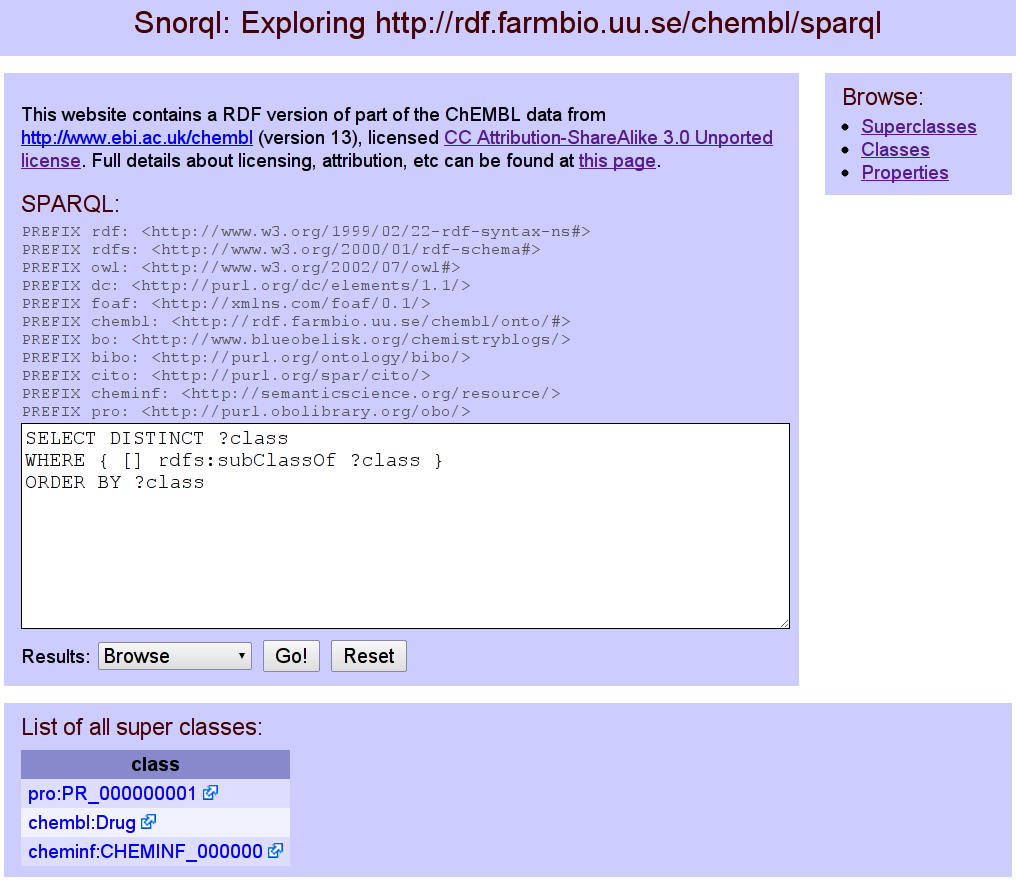
\includegraphics[width=0.45\textwidth]{snorql}
\caption{The SNORQL interface for browsing the SPARQL end point.}\label{f2}
\end{figure}

\section{Applications}

\subsection{Bio2RDF}

%Peter: write up the proxying... if that still works... It was broken through disuse, but is available again in its rdf.farmbio.uu.se configuration, separately from the bio2rdf-webapp at https://github.com/ansell/chembl-webapp/

The Bio2RDF project provides both resolvable Linked Data URIs using a generic Linked Data
server~\cite{Ansell2011} to access SPARQL endpoints for a range of scientific databases~\cite{Belleau2008}.
A number of these databases are referenced in ChEMBL, including ChEBI, Pubmed, and both the
Uniprot protein and taxonomy databases~\cite{TheUniProtConsortium2010}. These links are
vital to provide context for use cases that require a correlation between chemical
structures and other scientific data. 

The Linked Data server used by Bio2RDF has been reconfigured for ChEMBL to provide URL
based services for standard URI resolution, along with text and link searches
\cite{WebAppGitHub}. It proxies the standard item
URIs by translating URLs between those requested by users and the URIs that are available
in the databases. For example, if the ChEMBL web application is running on the users
local machine, e.g. \url{http://localhost:8080/chembl/}, then a request for the
article with identifier ``a31863'', \url{http://localhost:8080/-chembl/article/a31863},
will be resolved from the database using the full original URI,
\url{http://data.kasabi.com/-dataset/chembl-rdf/13/activity/a31863}. If the
user requested an RDF document, using content negotiation, the original URIs will be unchanged,
however, if the user requested an HTML document, the results will contain both the
original RDF triples, represented using RDFa, with links that resolve using the users local machine.

The links services enables the ChEMBL application to derive both forward links, originating in
ChEMBL, e.g. \url{http://localhost:8080/chembl/linkstonamespace/-targetns/originalns:identifier},
and backward links, originating in other databases, such as LODD, Bio2RDF, e.g.
\url{http://bio2rdf.org/linksns/targetns/originalns:ident-ifier}, or Chem2Bio2RDF.
These services are vital to efficiently navigate the Linked Data web, as it is both
impractical and inefficient to require users to crawl the web before they can discover all of the
relevant resources. These services are currently only supplied as web services from ChEMBL and
Bio2RDF, but it is hoped that similar services will be provided by other scientific Linked Data
providers in the future. Datasets that are available in SPARQL endpoints can be queried for
links efficiently using templated queries in the ChEMBL web application.

\subsection{CitedIn}

Andra: use the SPARQL end point to find which entries in ChEMBL cite what papers
 
The link between data and formal publication is important in many areas of
attribution, scientist ranking, etc, as outline in \cite{Waagmeester2012}.
ChEMBL contains many literature references, and we wish to query this data
for CitedIn.

\subsection{Decision Support}

Egon,Antony/Valery,Ola: develop and write up the Bioclipse Decision Support use case

\subsection{Chem2Bio2RDF}

David/Bin: Chem2Bio2RDF

\section{Discussion}

outlook ...

\section{Acknowledgements}

Tim Hodson and Zach Beauvais of Kasabi for their support. What S.H. Name of the Bioinformatics department at Uppsala University.

FIXME: add IMI

\bibliography{article}

%%%%%%%%%%% The bibliography starts:
%\begin{thebibliography}{9}
%
%\bibitem{r1}
%
%\bibitem{r2}
%
%\end{thebibliography}

\end{document}
